\documentclass{beamer}

%\usepackage[utf8x]{inputenc}
\usepackage{graphicx}
\usepackage{hyperref}
\usepackage{xspace}
\usepackage{amsmath}
\usetheme{Madrid}

\definecolor{pink}{rgb}{1.0,.8,.8}
\definecolor{hotpink}{cmyk}{0.0,0.8,0,0.2}
\definecolor{softred}{rgb}{.9,.7,.7}
\definecolor{darkred}{rgb}{.8,.1,.1}
\definecolor{purple}{rgb}{.7,.0,.7}
\definecolor{darkgreen}{rgb}{.1,.45,.1}
\definecolor{lightblue}{rgb}{0.3,0.3,1.0}
\definecolor{grey}{rgb}{.5,.5,.5}


\newcommand{\darkred}[1]{\textcolor{darkred}{#1}}
\newcommand{\darkgreen}[1]{\textcolor{darkgreen}{#1}}
\newcommand{\hotpink}[1]{\textcolor{hotpink}{#1}}
\newcommand{\lightblue}[1]{\textcolor{lightblue}{#1}}
\newcommand{\blue}[1]{\textcolor{blue}{#1}}
\newcommand{\red}[1]{\textcolor{red}{#1}}
\newcommand{\green}[1]{\textcolor{green}{#1}}
\newcommand{\purple}[1]{\textcolor{purple}{#1}}
\newcommand{\grey}[1]{\textcolor{grey}{#1}}
\newcommand{\MetDeltaPhi}{\Delta\phi(\MET, \rm{lepton, jet})}
\newcommand{\MET}{\mbox{$E\kern-0.50em\raise0.10ex\hbox{/}_{T}$}}
\newcommand{\met}{\ensuremath{E_T^{miss}}\xspace}
\newcommand{\metrel}{\ensuremath{E_{T}^{miss,~\mathrm{Rel}}}\xspace} 
\newcommand{\tmet}{\ensuremath{E_{T}^{miss,~\mathrm{Track}}}\xspace} 
\newcommand{\ptll}{\ensuremath{p_{T}^{\ell\ell}}\xspace} 
\newcommand{\ptg}{\ensuremath{p_{T}^{\gamma}}\xspace} 
\newcommand{\ptZ}{\ensuremath{p_{T}^{Z}}\xspace} 
\newcommand{\METsig}{\MET_{\mathrm{sig}}}
\newcommand{\delPhiMet}{\min{\Delta\phi(\MET,l\mathrm{~or~jet}))}} 
\newcommand{\dphill}{\ensuremath{\Delta\phi_{\ell\ell}}} 
\newcommand{\SumEt}{\sum{E_{T}}}
\newcommand{\nunubar}{\nu \overline{\nu}}
\newcommand{\ttbar}{t \overline{t}}
\newcommand{\ppbar}{p \overline{p}}
\newcommand{\qqbar}{q \overline{q}}
\newcommand{\bbbar}{b \overline{b}}
\newcommand{\epem}{ e^+e^-}
\newcommand{\pt}{\ensuremath{p_{T}}\xspace}
\newcommand{\HWW}{H\rightarrow WW}
\newcommand{\BR}[1]{{\cal{B}} (#1)}
\newcommand{\zzllnunu}{\ensuremath{ZZ\to\ell\ell\nu\nu}\;}

\newcommand {\Dzero} {D\O\ }

\newcommand {\rmfrac}[2]{ $\frac{\mathrm{#1}}{\mathrm{#2}}$ }

\newcommand{\bc}{\begin{columns}}
\newcommand{\ec}{\end{columns}}
\newcommand{\fr}[2]{\begin{frame} \frametitle{#1} #2 \end{frame} }


\newcommand{\figbox}[5][]{
   \parbox{#2\textwidth}{
   \centering
   \includegraphics[#1,width=#3\textwidth]{#4}
   \ifthenelse{ \equal{}{#5} } {} {\\ #5}
}} 

\newcommand{\figboxv}[4]{
   \parbox{#1\textwidth}{
   \begin{center}
   \includegraphics[height=#2\textwidth]{#3}   
   \ifthenelse{ \equal{}{#4} } {} {
     \vspace{-0.35cm}
     \begin{center}
       #4
     \end{center}
   }
   \end{center}
}} 



\title[ $W\gamma\gamma$ ]
{ $W\gamma\gamma$ }

\author[Josh Kunkle]
  {Josh Kunkle, Alberto Belloni, Chris Anelli}

\institute[UMD]{University of Maryland}

\date[August 15, 2013] % (optional)
{ 
  \vspace{0.5cm} \begin{center}\includegraphics[width=0.3\textwidth]{../UMDLogo.pdf}\end{center}
  \vspace{0.5cm}
}

\begin{document}

\maketitle

\fr{ Fiducial definition } {

    \blue{See Alberto's talk}

    \[
    \frac{N_{obs} - N_{bkg}}{\mathcal{L}} = \sigma_{fid.} \times C_{WAA} = \sigma_{tot.} \times A_{WAA} \times C_{WAA}
    \]

    \begin{itemize}
        \item $C_{WAA}$ = reconstruction efficiency within the fiucial volume
        \item $A_{WAA}$ = acceptance of the fiducial volume
    \end{itemize}

    \[
        C_{WAA} = \frac{N_{MC}^{reco.}}{N_{MC}^{gen, fiducial}} \times \frac{\epsilon^{data}}{\epsilon^{MC}}
    \]
    \[
        A_{WAA} = \frac{N_{MC}^{gen, fiducial}}{N_{MC}^{gen, total}}
    \]

    \red{NB - because we have photons in the event, $N_{MC}^{gen, total}$ must also be defined by a minimum photon \pt cut}

}

\fr{ Fiducial definition }{ 

    Should closely mimic the reconstruction cuts.  Check this once reconstruction cuts are determined.

    \vspace{4mm}

    \begin{itemize}
        \item One $e$ or $\mu$ having $\pt > 25$ GeV, $|\eta| < 2.5$ (can orignate from a $\tau$)
        \item Two photons having $\pt > 15$ GeV, $|\eta| < 2.5$
        \item Objects should not overlap, $\Delta R(\gamma, \ell) > 0.2$, $\Delta R(\gamma, \gamma) > 0.2$
        \item Any additional background rejection cuts ($m_{T}$, $p_{T}^{\nu}$)
    \end{itemize}

}

\fr{ Comparing ISR to FSR } {

    \begin{itemize}
        \item Expect kinematics to differ between ISR and FSR enhanced samples
    \end{itemize}

    \vspace{4mm}

    \begin{figure}
        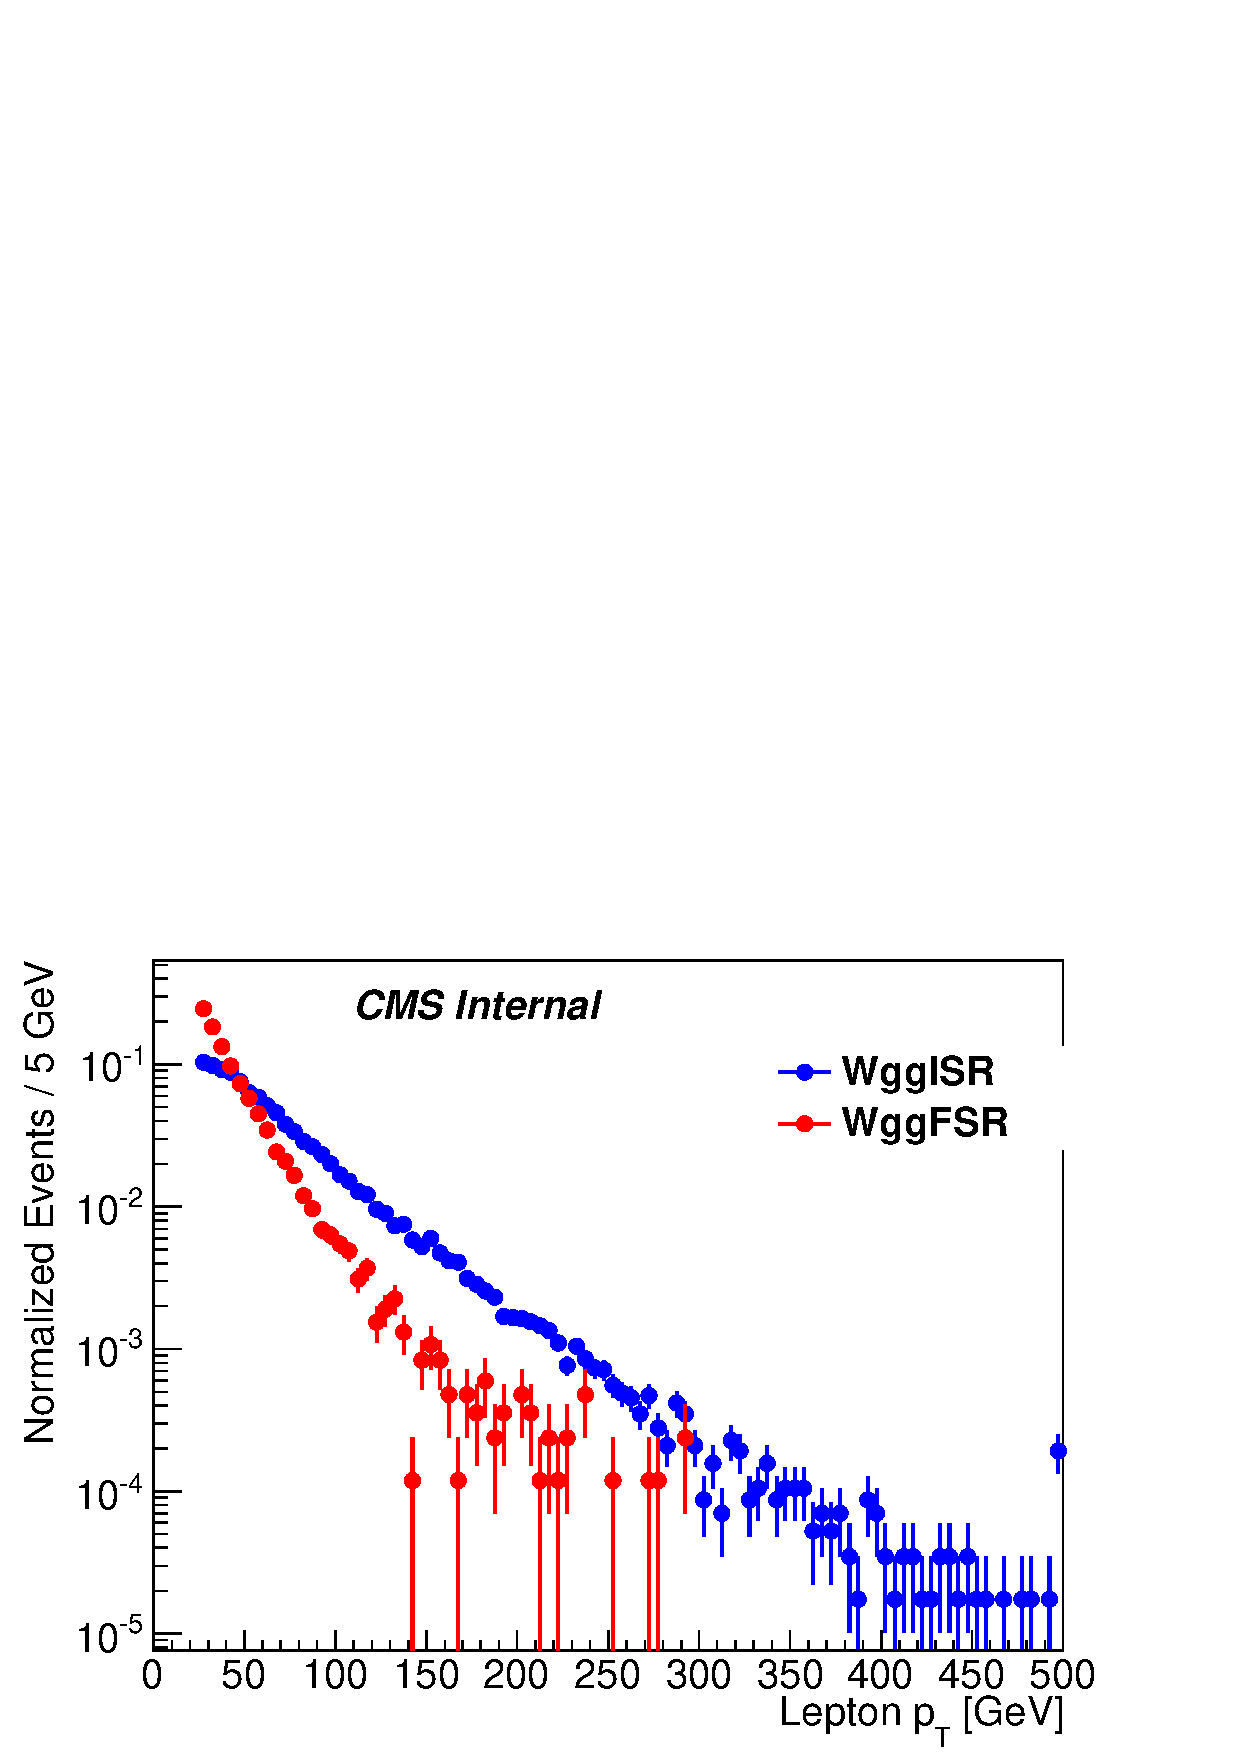
\includegraphics[width=0.33\textwidth]{Plots/lep_pt_1l2p.pdf}
        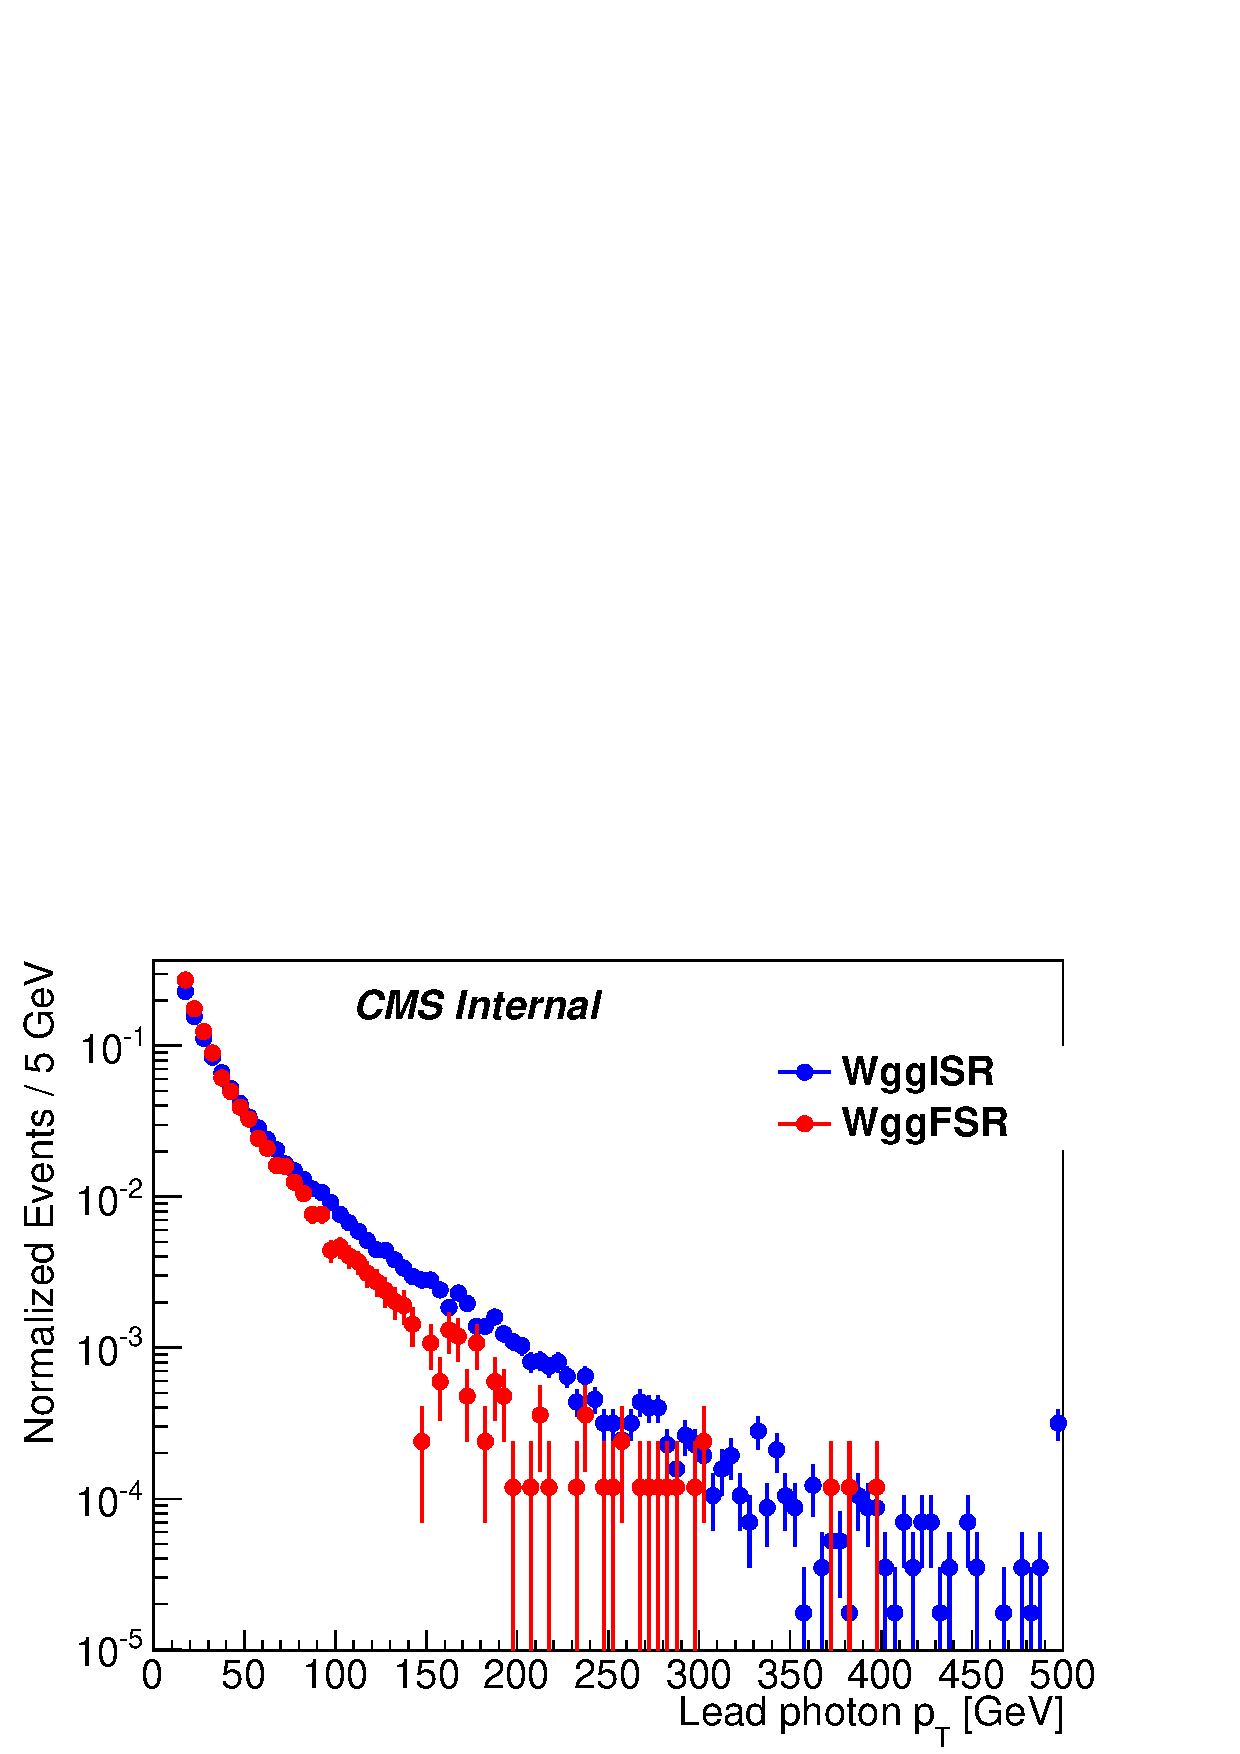
\includegraphics[width=0.33\textwidth]{Plots/lead_phot_pt_1l2p.pdf}
        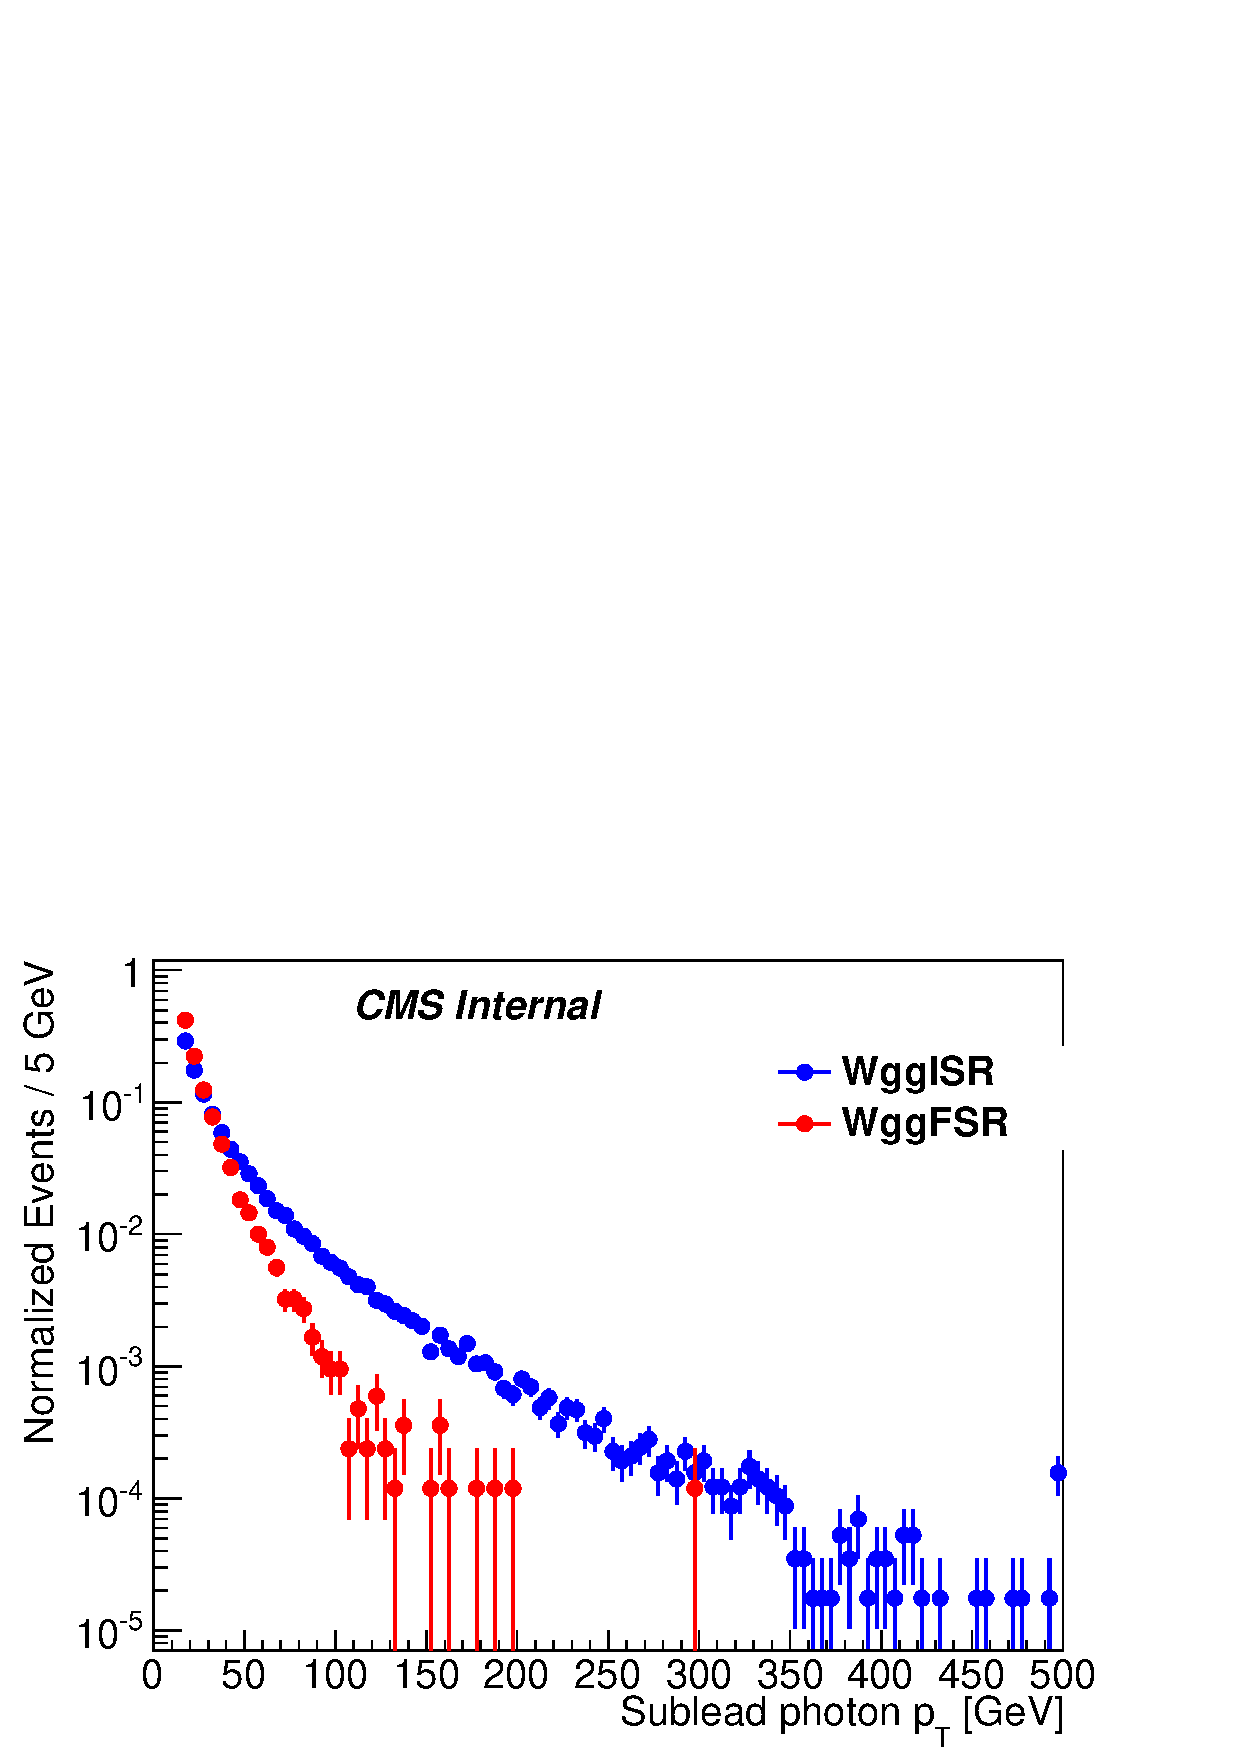
\includegraphics[width=0.33\textwidth]{Plots/subl_phot_pt_1l2p.pdf}
    \end{figure}

    

}

\fr{ Comparing ISR to FSR } {

    \begin{itemize}
        \item We must require overlap removal at the truth level.  Check these distributions
    \end{itemize}

    \begin{figure}
        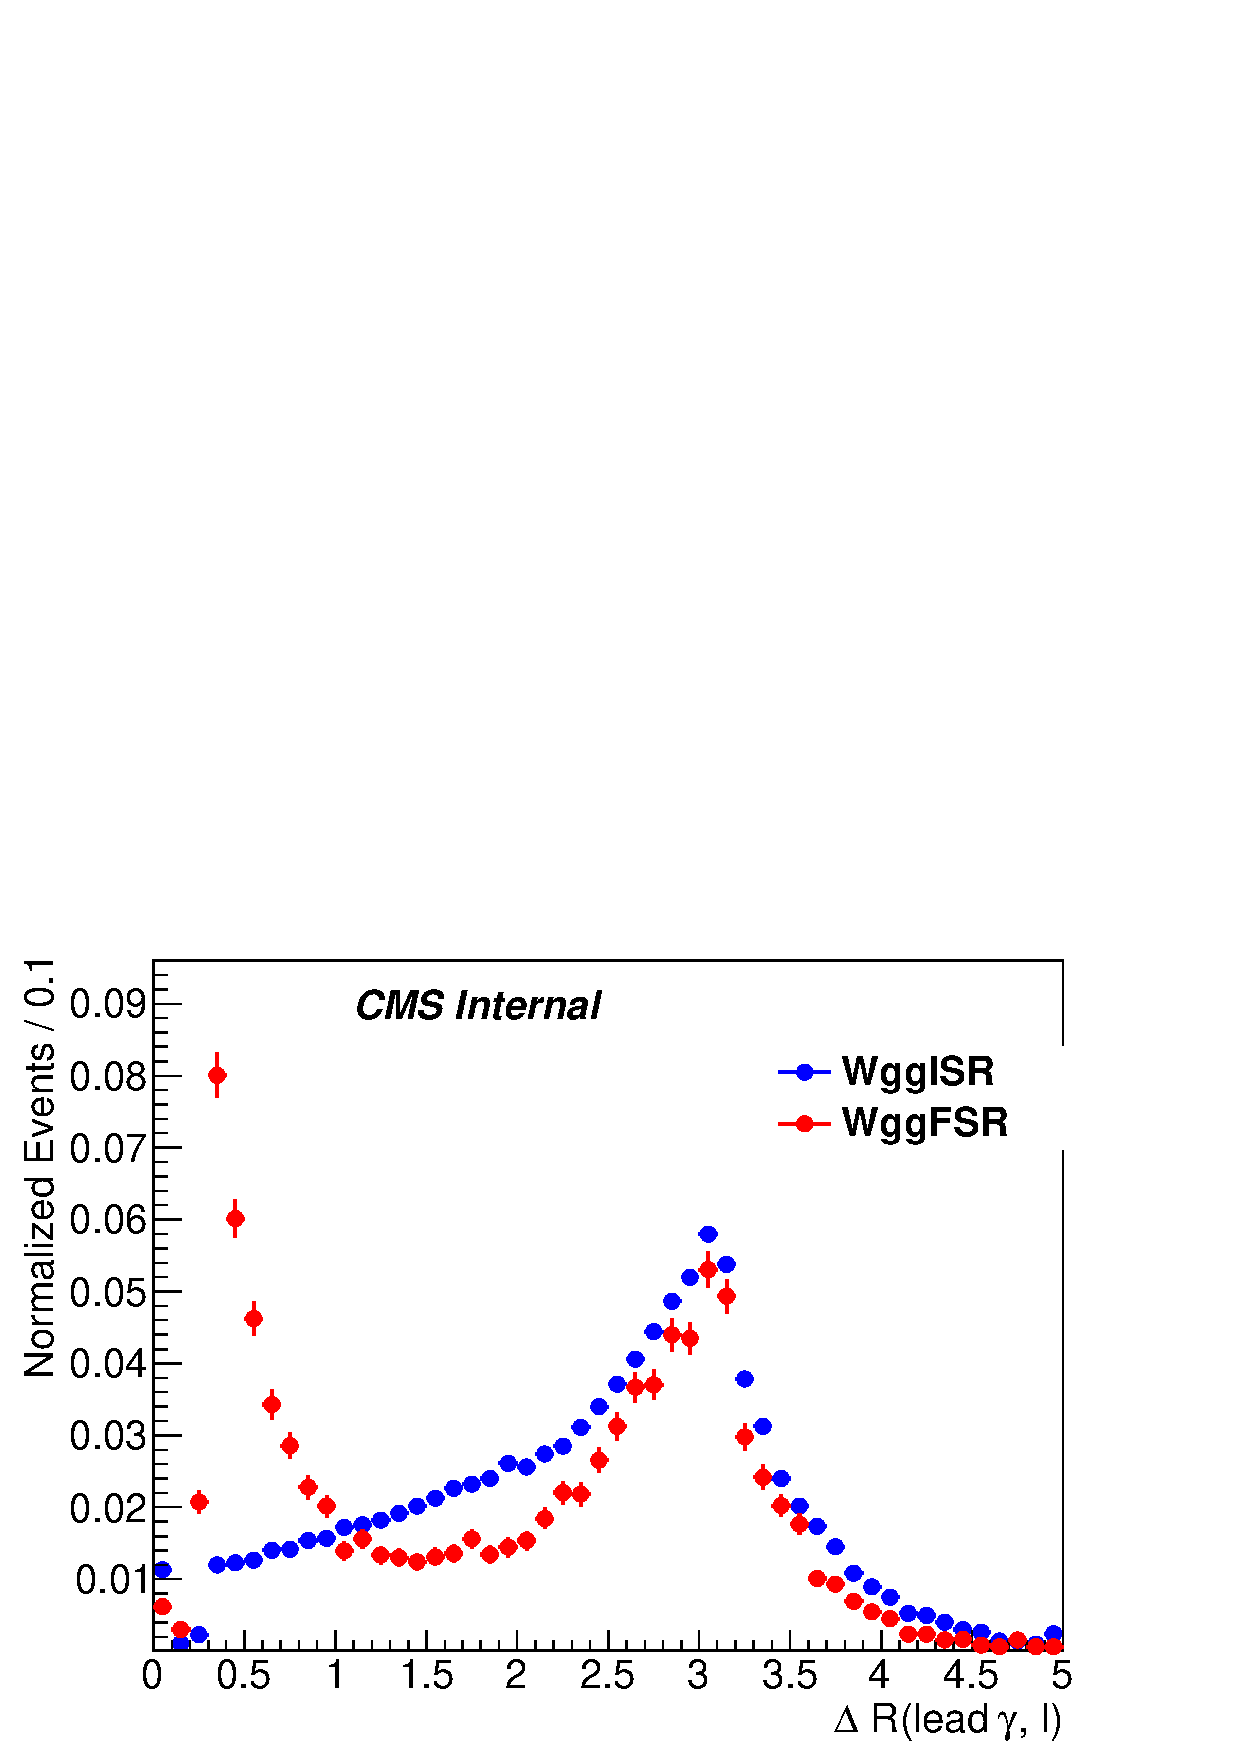
\includegraphics[width=0.33\textwidth]{Plots/lead_phot_lepDR_1l2p.pdf}
        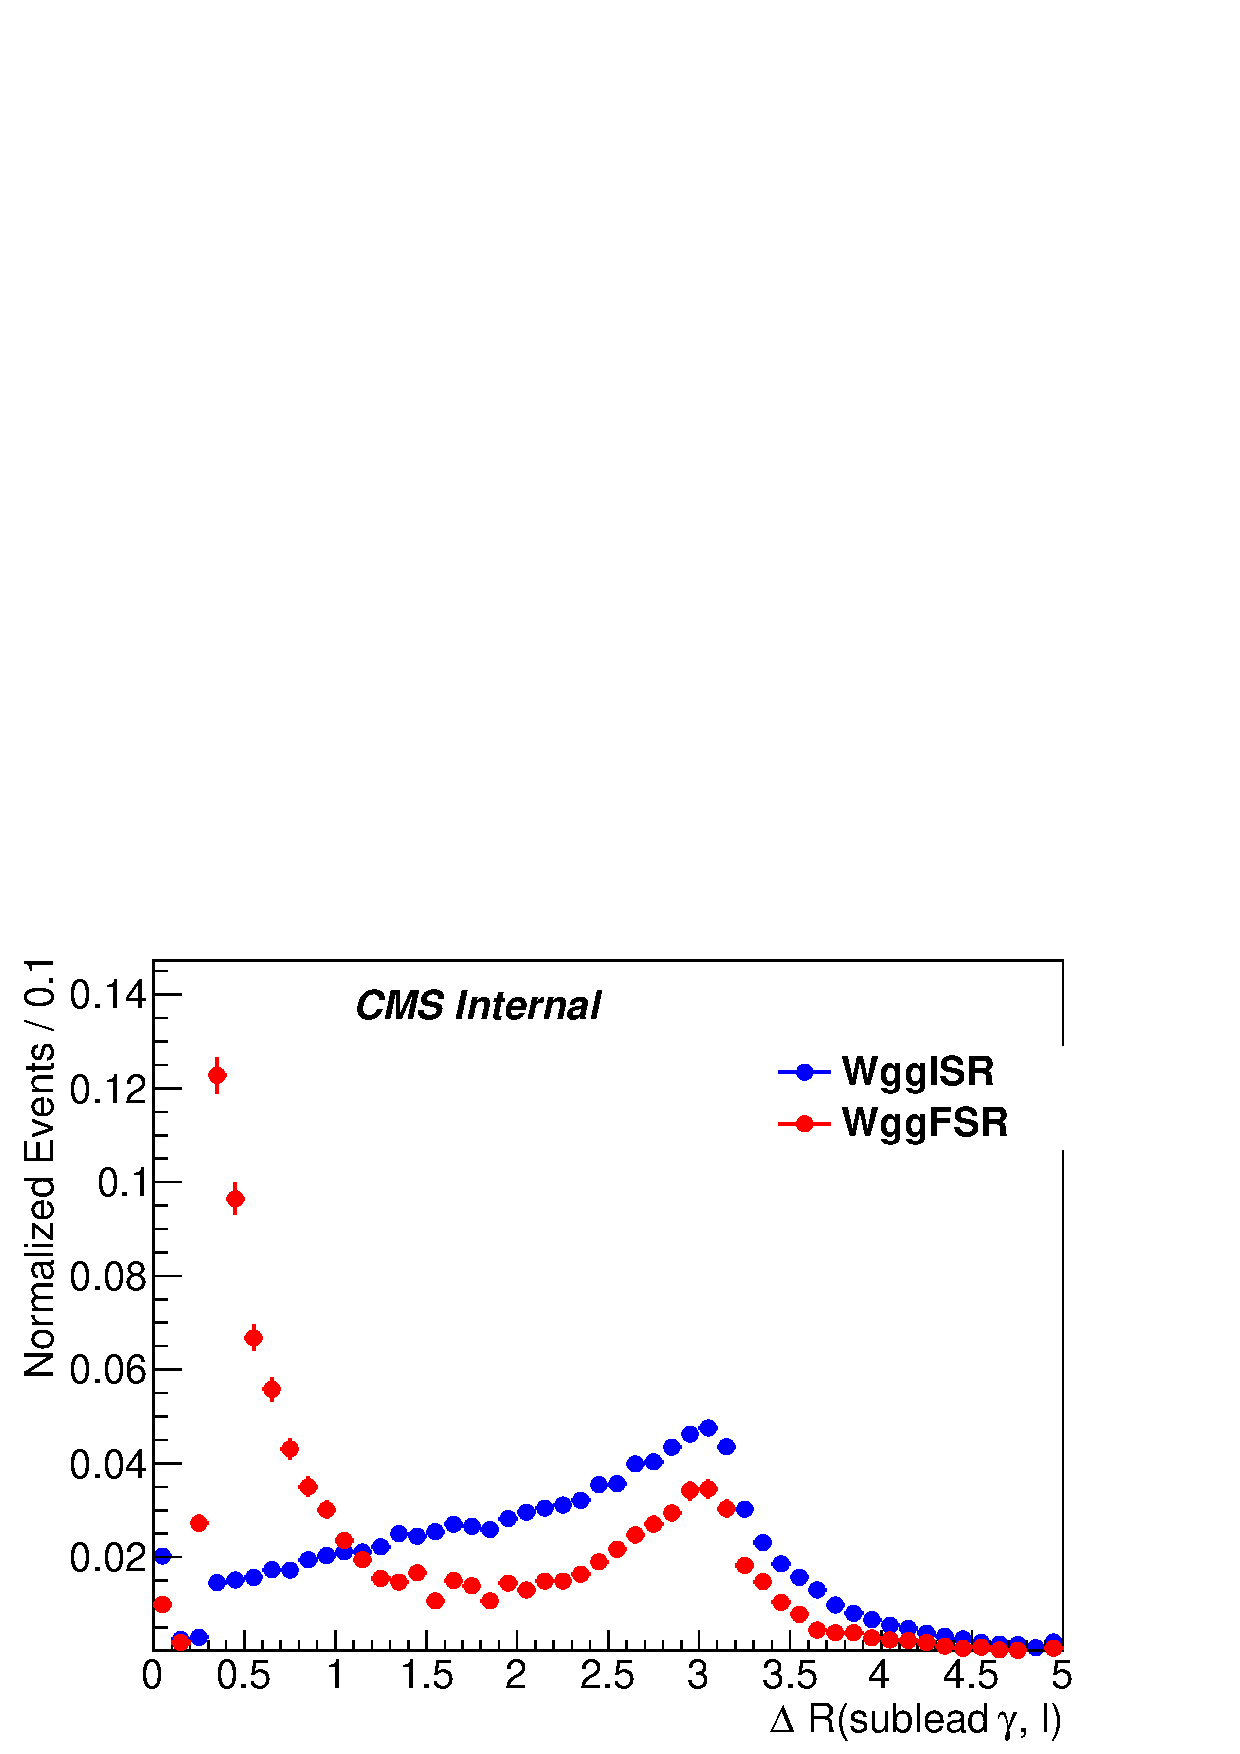
\includegraphics[width=0.33\textwidth]{Plots/subl_phot_lepDR_1l2p.pdf}
        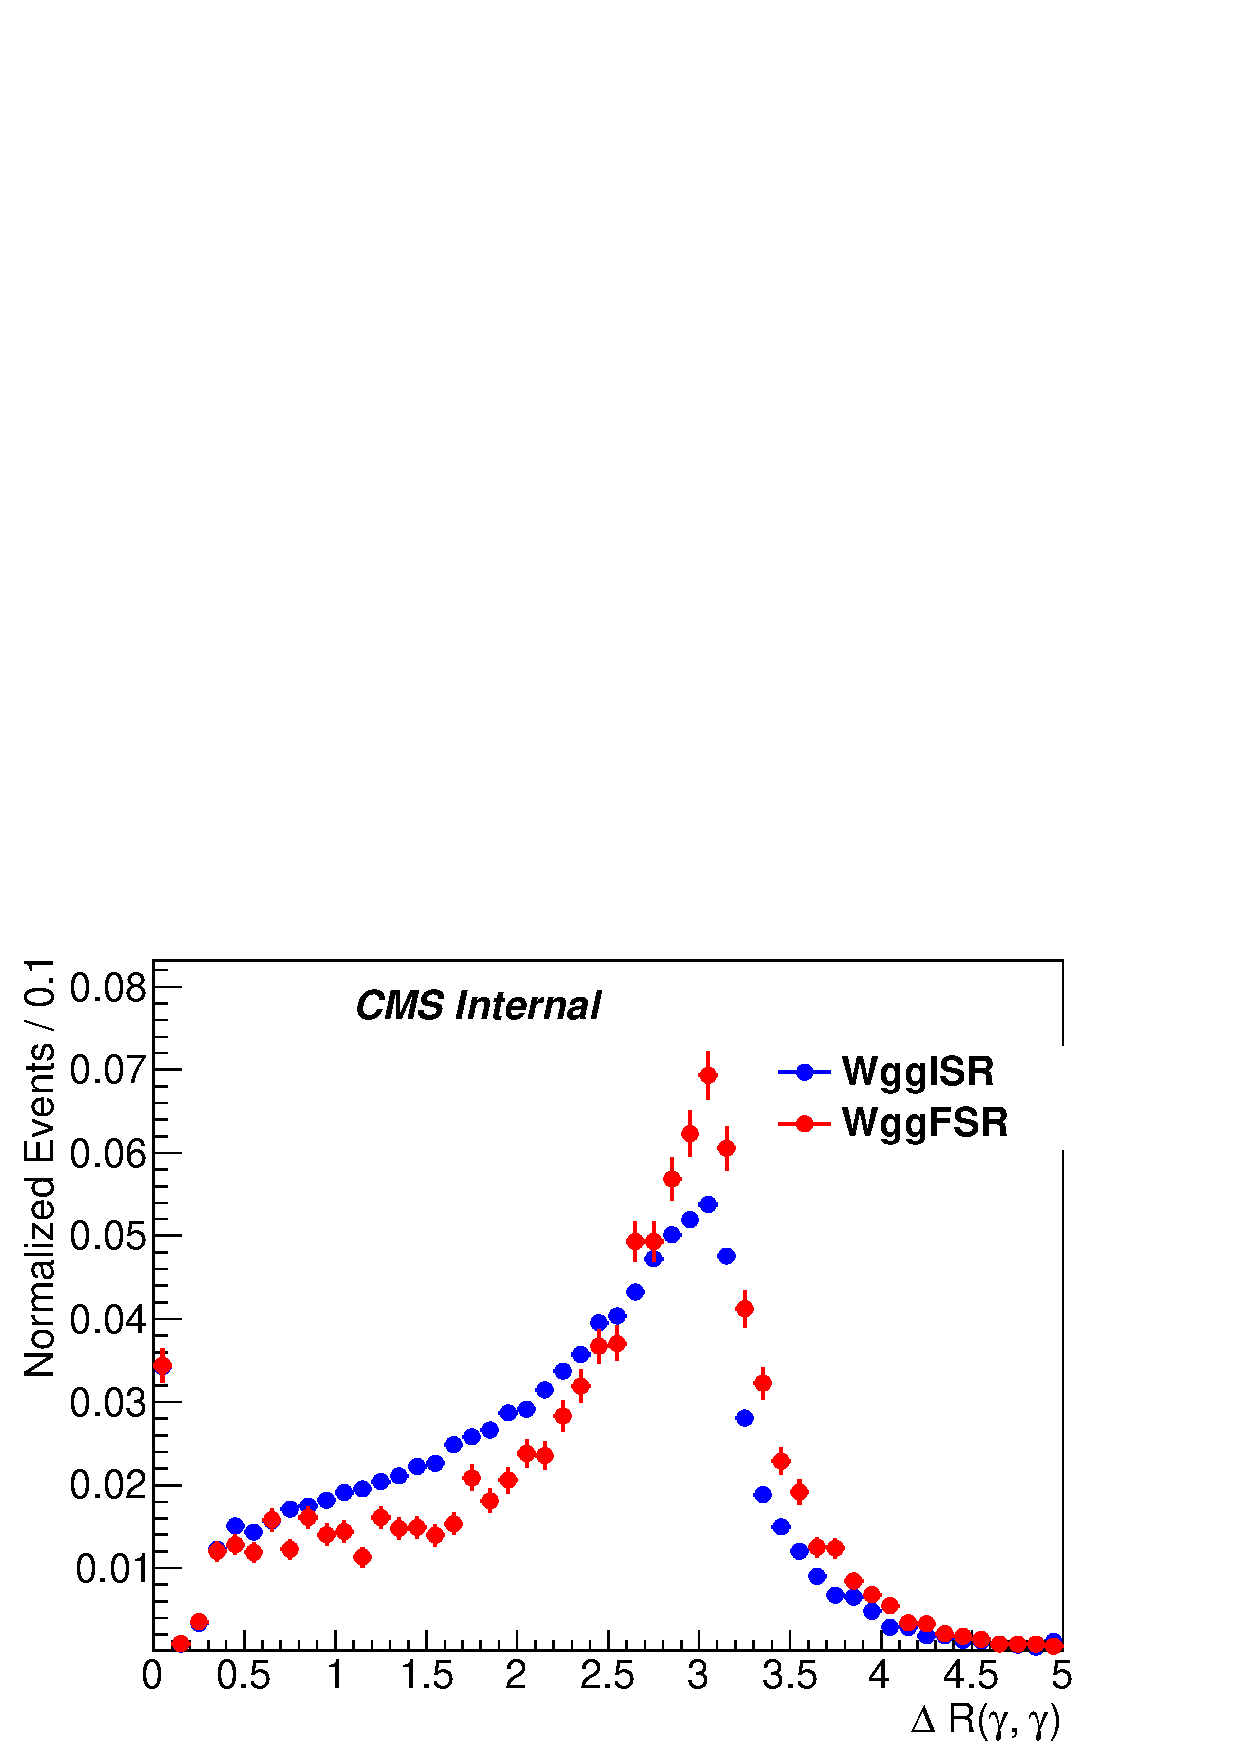
\includegraphics[width=0.33\textwidth]{Plots/phot_photDR_1l2p.pdf}
    \end{figure}

}

\fr{ Comparing ISR to FSR } {
    
    \begin{itemize}
        \item Additional background rejection cuts ($m_{T}$, \met ( $p_{T}^{\nu}$ ) )
    \end{itemize}

    \begin{figure}
        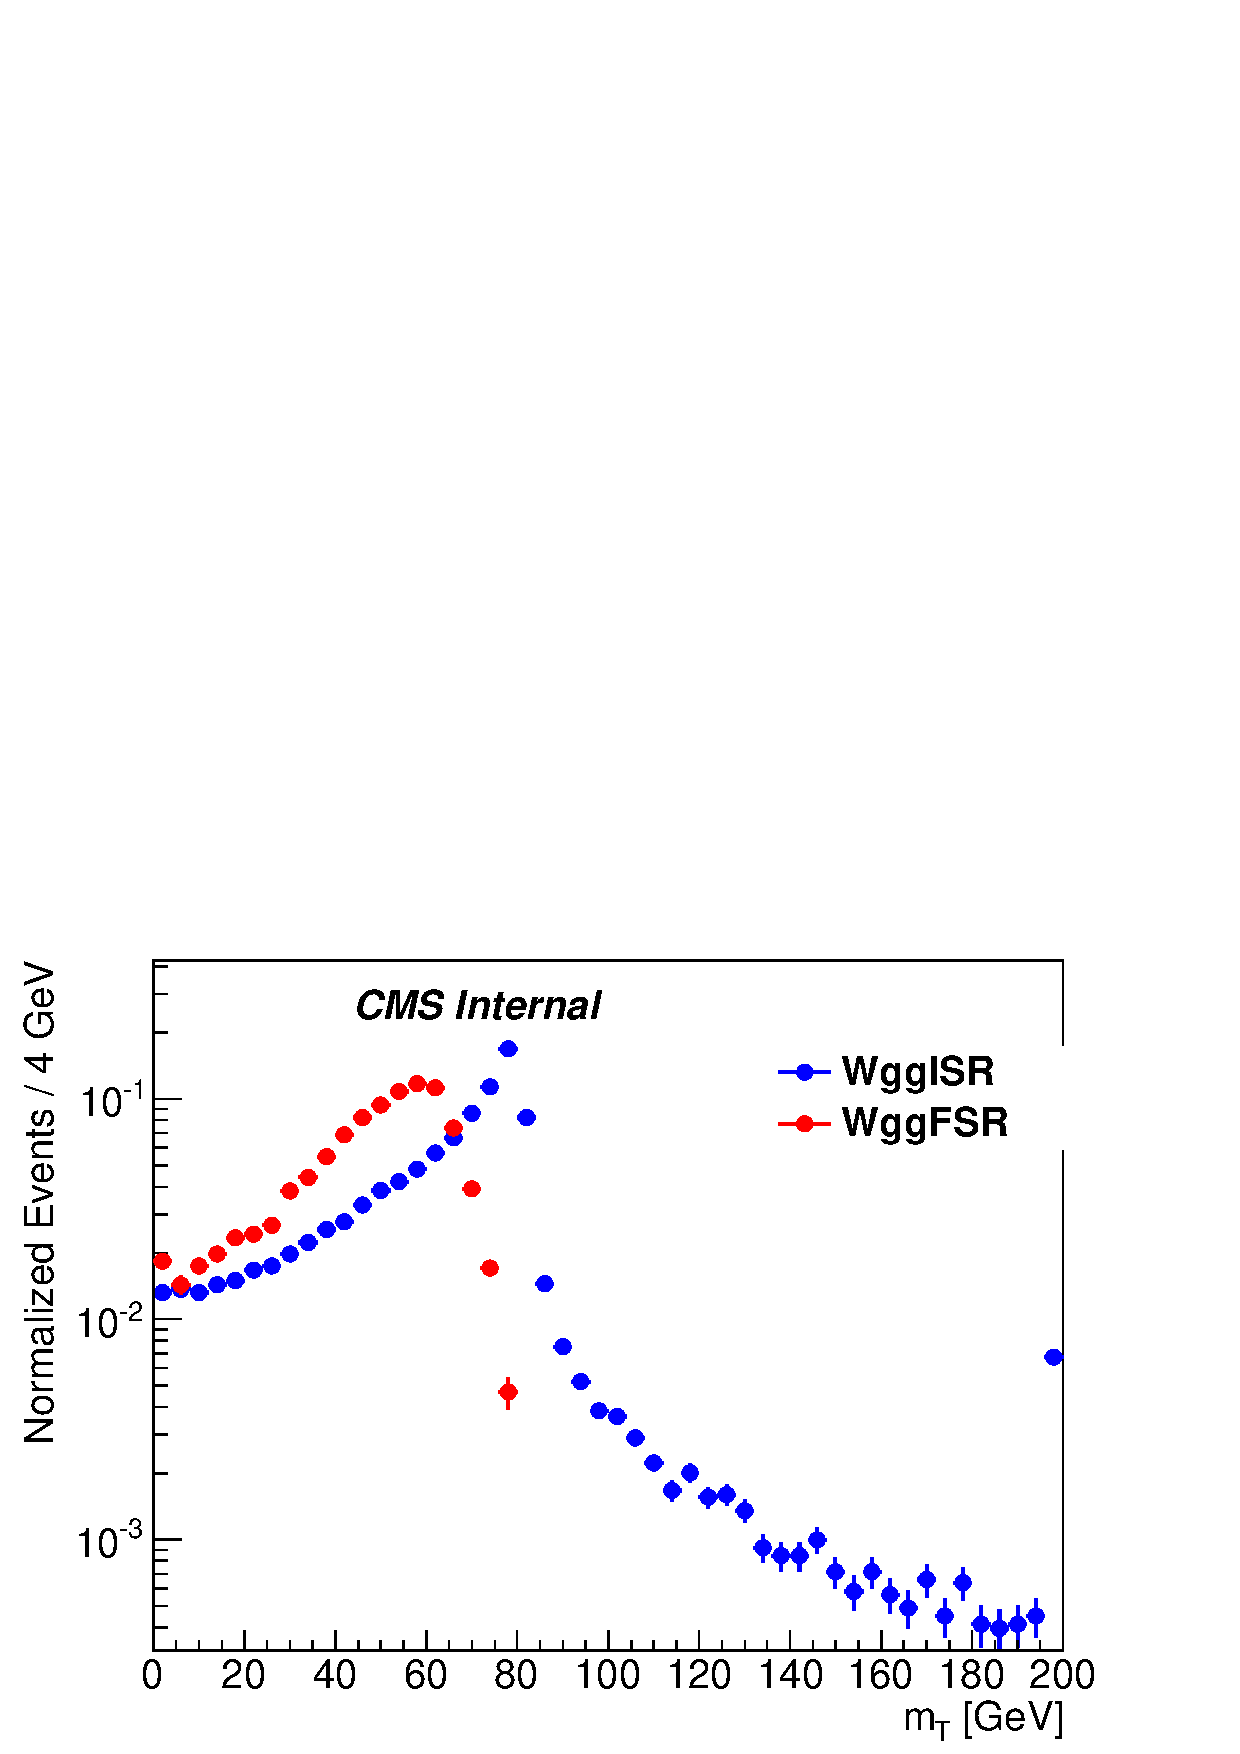
\includegraphics[width=0.45\textwidth]{Plots/mt_1l2poverlap.pdf}
        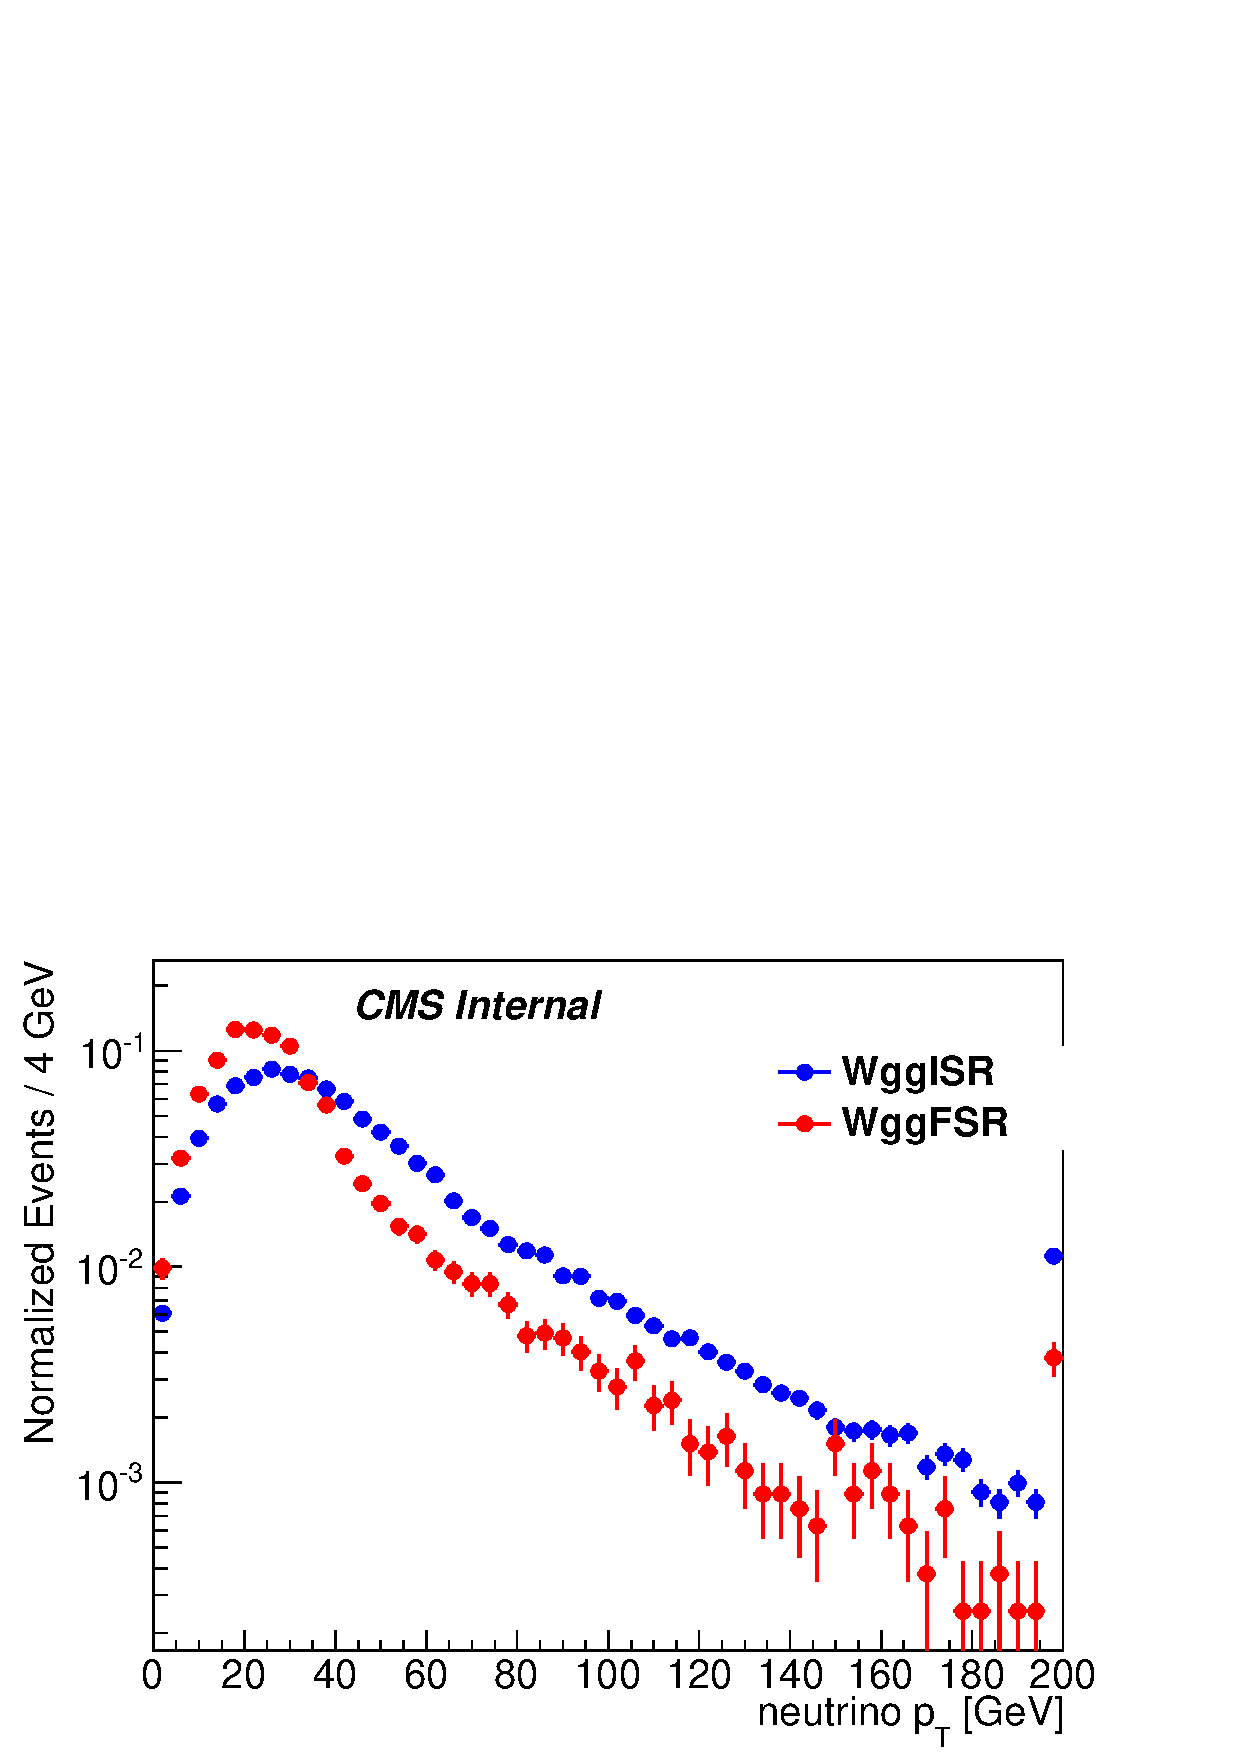
\includegraphics[width=0.45\textwidth]{Plots/met_1l2poverlap.pdf}
    \end{figure}

}

\fr{ Acceptances } {

    \begin{itemize}
        \item Acceptances should be different for the FSR and ISR enhanced samples
    \end{itemize}

    \vspace{4mm}
  
    \tiny

    \begin{tabular}{| l | c | c | c | c | c | c | }
    Cuts         & WggISR            & Acceptance           & WggFSR            & Acceptance               & Combined          & Acceptance      \\  \hline
    One Lepton   & 422782 & 0.4211 $\pm$ 0.0008  & 116125  & 0.1161 $\pm$ 0.0004      & 538907  & 0.2689 $\pm$ 0.0004 \\ 
    Two Photons  & 57252  & 0.0570 $\pm$ 0.0002  & 8393    & 8.390e-03 $\pm$ 9.2e-05  & 65645   & 0.0328 $\pm$ 0.0001 \\ 
    Overlap Rm   & 53240  & 0.0530 $\pm$ 0.0002  & 7922    & 7.920e-03 $\pm$ 8.9e-05  & 61162   & 0.0305 $\pm$ 0.0001 \\ 
    $m_{T} >$ 40 & 44124  & 0.0440 $\pm$ 0.0002  & 5691    & 5.689e-03 $\pm$ 7.6e-05  & 49815   & 0.0249 $\pm$ 0.0001 \\ 
     \end{tabular}

    \vspace{5mm}

    \centering
      \large
        $A_{WAA} = 0.03$ before additional background rejection cuts


}

\fr{ Lepton acceptances } {

    \begin{itemize}
        \item The total acceptance is a combination of $W\to e, \mu$ and $W\to \tau \to e, \mu$.  However
          tau decays produce lower \pt leptons and thus have lower acceptance
    \end{itemize}


        
    Only $W\to e, \mu$

    \vspace{2mm}

    \tiny
    \begin{tabular}{| l | c | c | c | c | c | c | }
    Cuts         & WggISR            & Acceptance           & WggFSR            & Acceptance           & Combined          & Acceptance \\ 
    One Lepton   & 404854  & 0.605 $\pm$ 0.001    & 113931  & 0.1597 $\pm$ 0.0005  & 518785  & 0.3751 $\pm$ 0.0006 \\ 
    Two Photons  & 54090   & 0.0808 $\pm$ 0.0004  & 8133    & 0.0114 $\pm$ 0.0001  & 62223   & 0.0450 $\pm$ 0.0002 \\ 
    Overlap Rm   & 50253   & 0.0751 $\pm$ 0.0003  & 7680    & 0.0108 $\pm$ 0.0001  & 57933   & 0.0419 $\pm$ 0.0002 \\ 
    $m_{T} >$ 40 & 42150   & 0.0629 $\pm$ 0.0003  & 5555    & 0.0078 $\pm$ 0.0001  & 47705   & 0.0345 $\pm$ 0.0002 \\ 
     \end{tabular}

    \vspace{2mm}


    \normalsize
    Only $W\to \tau$ (BR $tau\to \ell$ = 35\%)

    \vspace{2mm}

    \tiny

    \begin{tabular}{| l | c | c | c | c | c | c | }
    Cuts         & WggISR           & Acceptance           & WggFSR         & Acceptance               & Combined         & Acceptance \\ 
    One Lepton   & 17928   & 0.0536 $\pm$ 0.0004  & 2194  & 0.0077 $\pm$ 0.0002      & 20122 & 0.0325 $\pm$ 0.0002 \\ 
    Two Photons  & 3162    & 0.0095 $\pm$ 0.0002  & 260   & 9.150e-04 $\pm$ 5.7e-05  & 3422  & 5.533e-03 $\pm$ 9.5e-05 \\ 
    Overlap Rm   & 2987    & 0.0089 $\pm$ 0.0002  & 242   & 8.516e-04 $\pm$ 5.5e-05  & 3229  & 5.221e-03 $\pm$ 9.2e-05 \\ 
    $m_{T} >$ 40 & 1974    & 0.0059 $\pm$ 0.0001  & 136   & 4.786e-04 $\pm$ 4.1e-05  & 2110  & 3.412e-03 $\pm$ 7.4e-05 \\ 
     \end{tabular}

    \begin{center}
        \large
        $A_{WAA} = 0.042$ for $W\to e, \mu$

        $A_{WAA} = 0.0052$ for $W\to \tau$, 0.015 for $W\to \tau \to e, \mu$
    \end{center}
}

\fr{ TGC and QGC acceptances } {


    \begin{itemize}
        \item Check how acceptances differ between QGC, TGC, and remaining events
        \item Require 0, 1, or 2 photons to have a W as a mother
    \end{itemize}

    \vspace{4mm}

    \begin{center}
    \scriptsize
    \begin{tabular}{l | c | c | c | }
        Sample & 2 W photons & 1 W photons & 0 W photons \\ \hline

          FSR  & 14112 & 294051 & 692147 \\ 
          ISR  & 13    &  13238 & 990669 \\
     \end{tabular}
    \end{center}

    \vspace{2mm}

    \normalsize
    Combine FSR and ISR samples below

    \vspace{2mm}

    \tiny
    \begin{tabular}{| l | c | c | c | c | c | c | }
          Cuts         & 0 W photons       & Acceptance           & 1 W photons      & Acceptance           & 2 W photons   & Acceptance         \\  \hline
          One Lepton   & 511314  & 0.3038 $\pm$ 0.0005  & 27105  & 0.0882 $\pm$ 0.0006  & 488  & 0.035 $\pm$ 0.002  \\ 
          Two Photons  & 57226   & 0.0340 $\pm$ 0.0001  & 7998   & 0.0260 $\pm$ 0.0003  & 421  & 0.030 $\pm$ 0.001  \\ 
          Overlap Rm   & 52825   & 0.0314 $\pm$ 0.0001  & 7926   & 0.0258 $\pm$ 0.0003  & 411  & 0.029 $\pm$ 0.001  \\ 
          $m_{T} >$ 40 & 43740   & 0.0260 $\pm$ 0.0001  & 5841   & 0.0190 $\pm$ 0.0003  & 234  & 0.017 $\pm$ 0.001  \\ 
     \end{tabular}

}


\end{document}

